\documentclass[1_relazione.tex]{subfiles}
\begin{document}
    \section{Test e validazione}\label{sec:test-e-validazione}
    Per verificare che il nostro sito sia valido ed accessibile a tutte le categorie degli utenti, sono stati usati i seguenti strumenti.

    \subsection{Total Validator}
    Usato per validare le pagine HTML generate dalle pagine HTML.\newline
    Risultato: \textbf{tutte le pagine sono valide}.
    \subsection{W3C HTML Validator}
    Come fonte pi\`{u} autorevole, \`{e} stato usato il validatore del W3C.\newline
    Risultato: \textbf{tutte le pagine sono valide}.
    \subsection{W3C CSS Validator}
    Usato per verificare la validit\`{a} dei fogli di stile CSS. \newline
    Risultato: \textbf{main.css e print.css sono entrambi validi}.
    \subsection{WAVE}
    Usato per effettuare la valutazione di accessibilit\`{a} del sito con un risultato: \textbf{nessun errore generico e nessun errore di contrasto}.
    \\Segnala un falso positivo quando nella schermata ci sono dei messaggi di errore di color rosso, mentre provando con altri strumenti, come il sito:\\ \url{https://www.colorblindness.com/coblis-color-blindness-simulator/}
    e l'estensione \textit{Colorblinding} per Chrome, il problema non sussiste.
    \begin{figure}[h!]
        \centering
        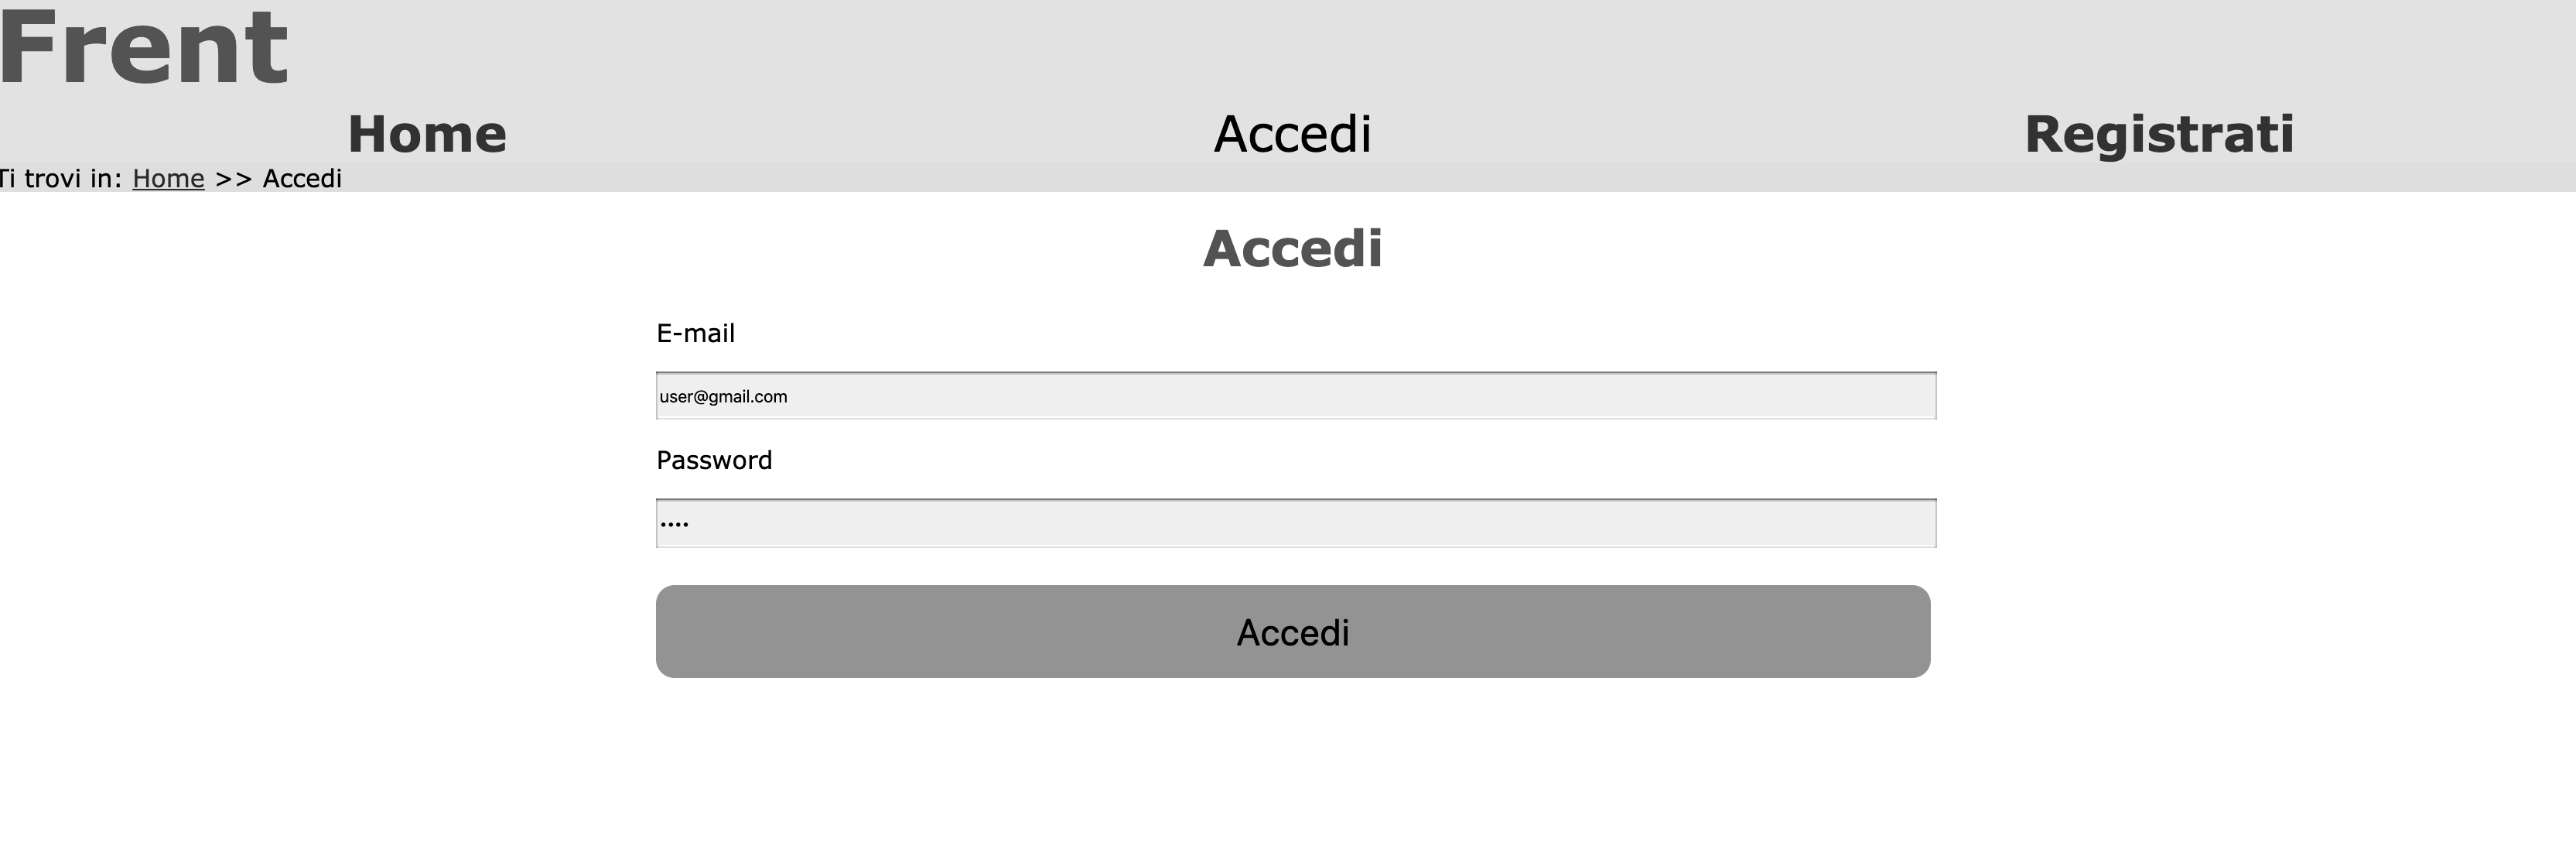
\includegraphics[scale=0.27]{immagini/Achromatopsia.png}
        \caption{il sito visto da chi \`{e} affetto da acromatopsia}
    \end{figure}
    \begin{figure}[h!]
        \centering
        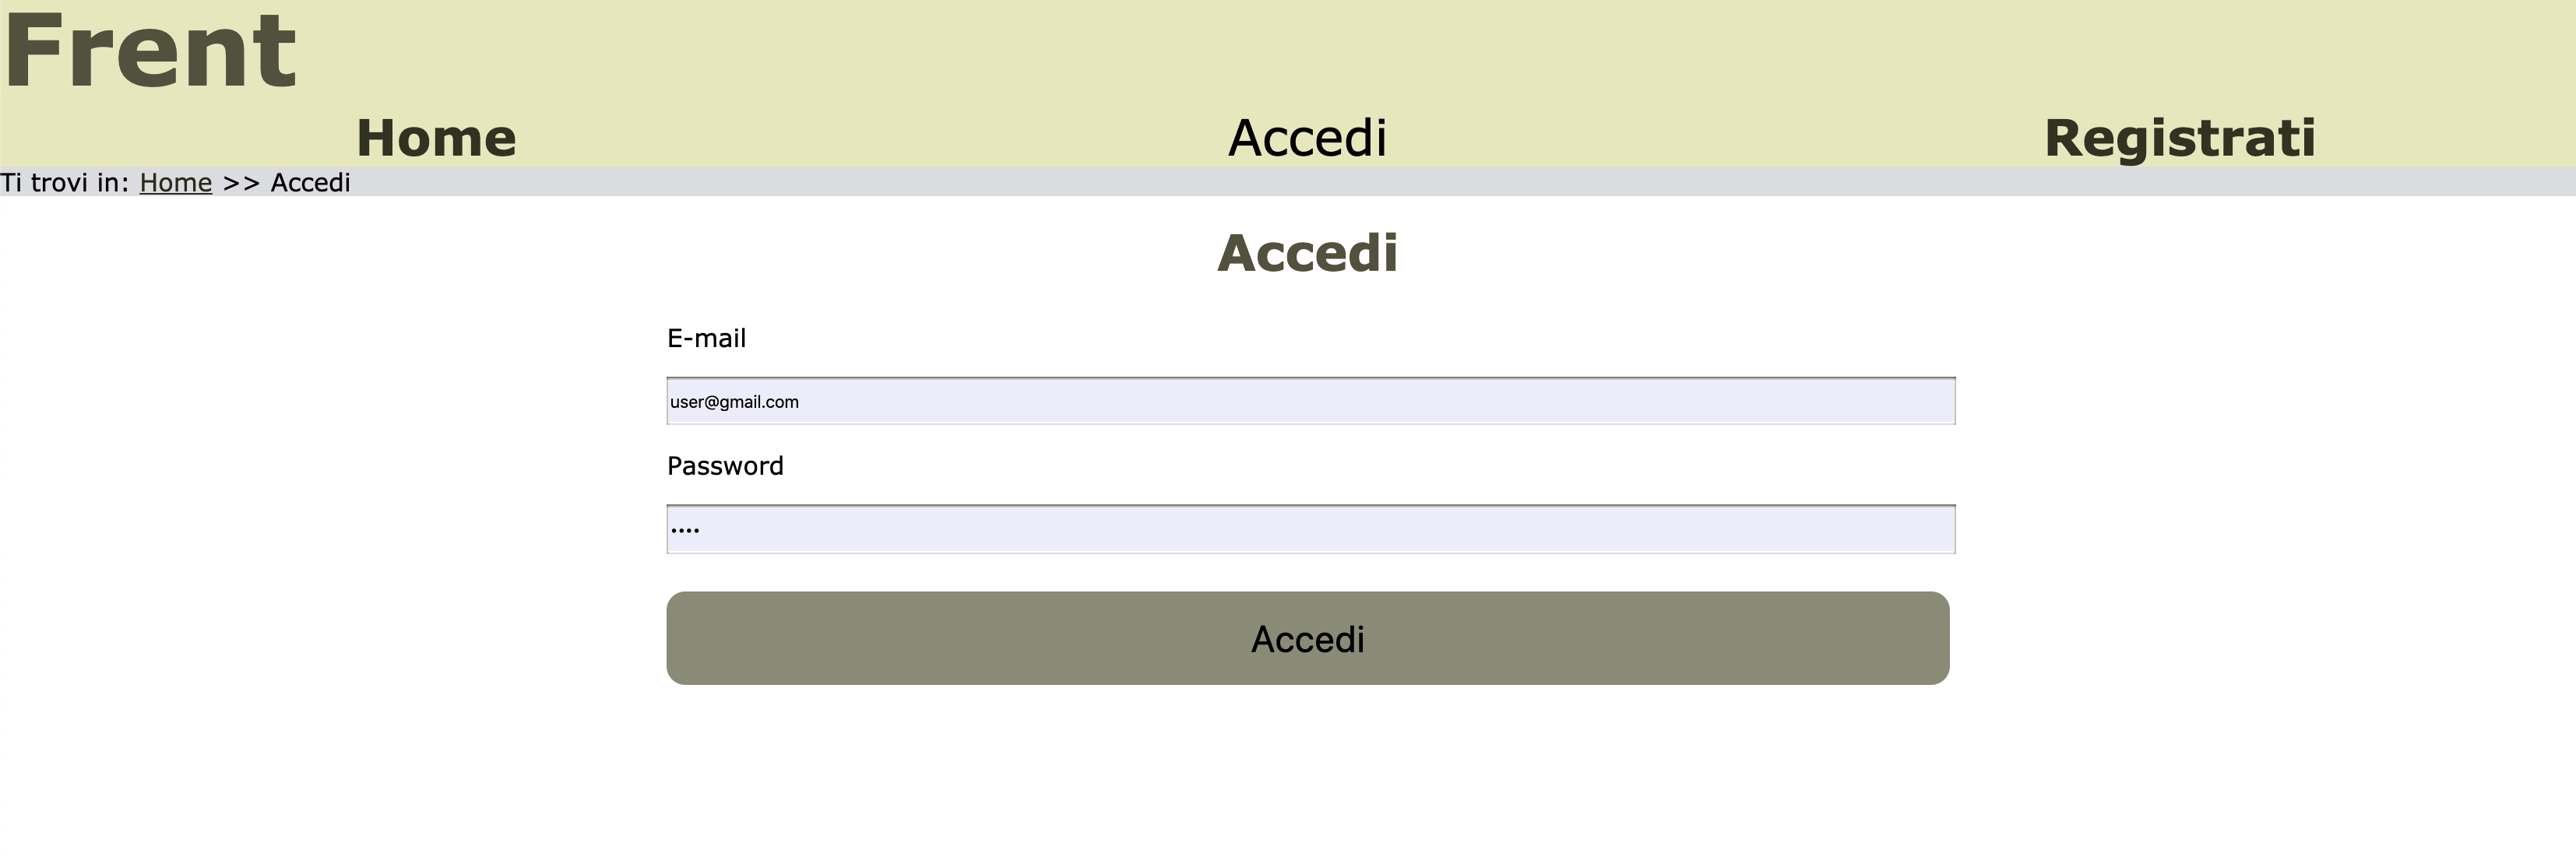
\includegraphics[scale=0.27]{immagini/Protanopia.png}
        \caption{il sito visto da chi \`{e} affetto da protanopia}
    \end{figure}
    \newpage
    \begin{figure}[h!]
        \centering
        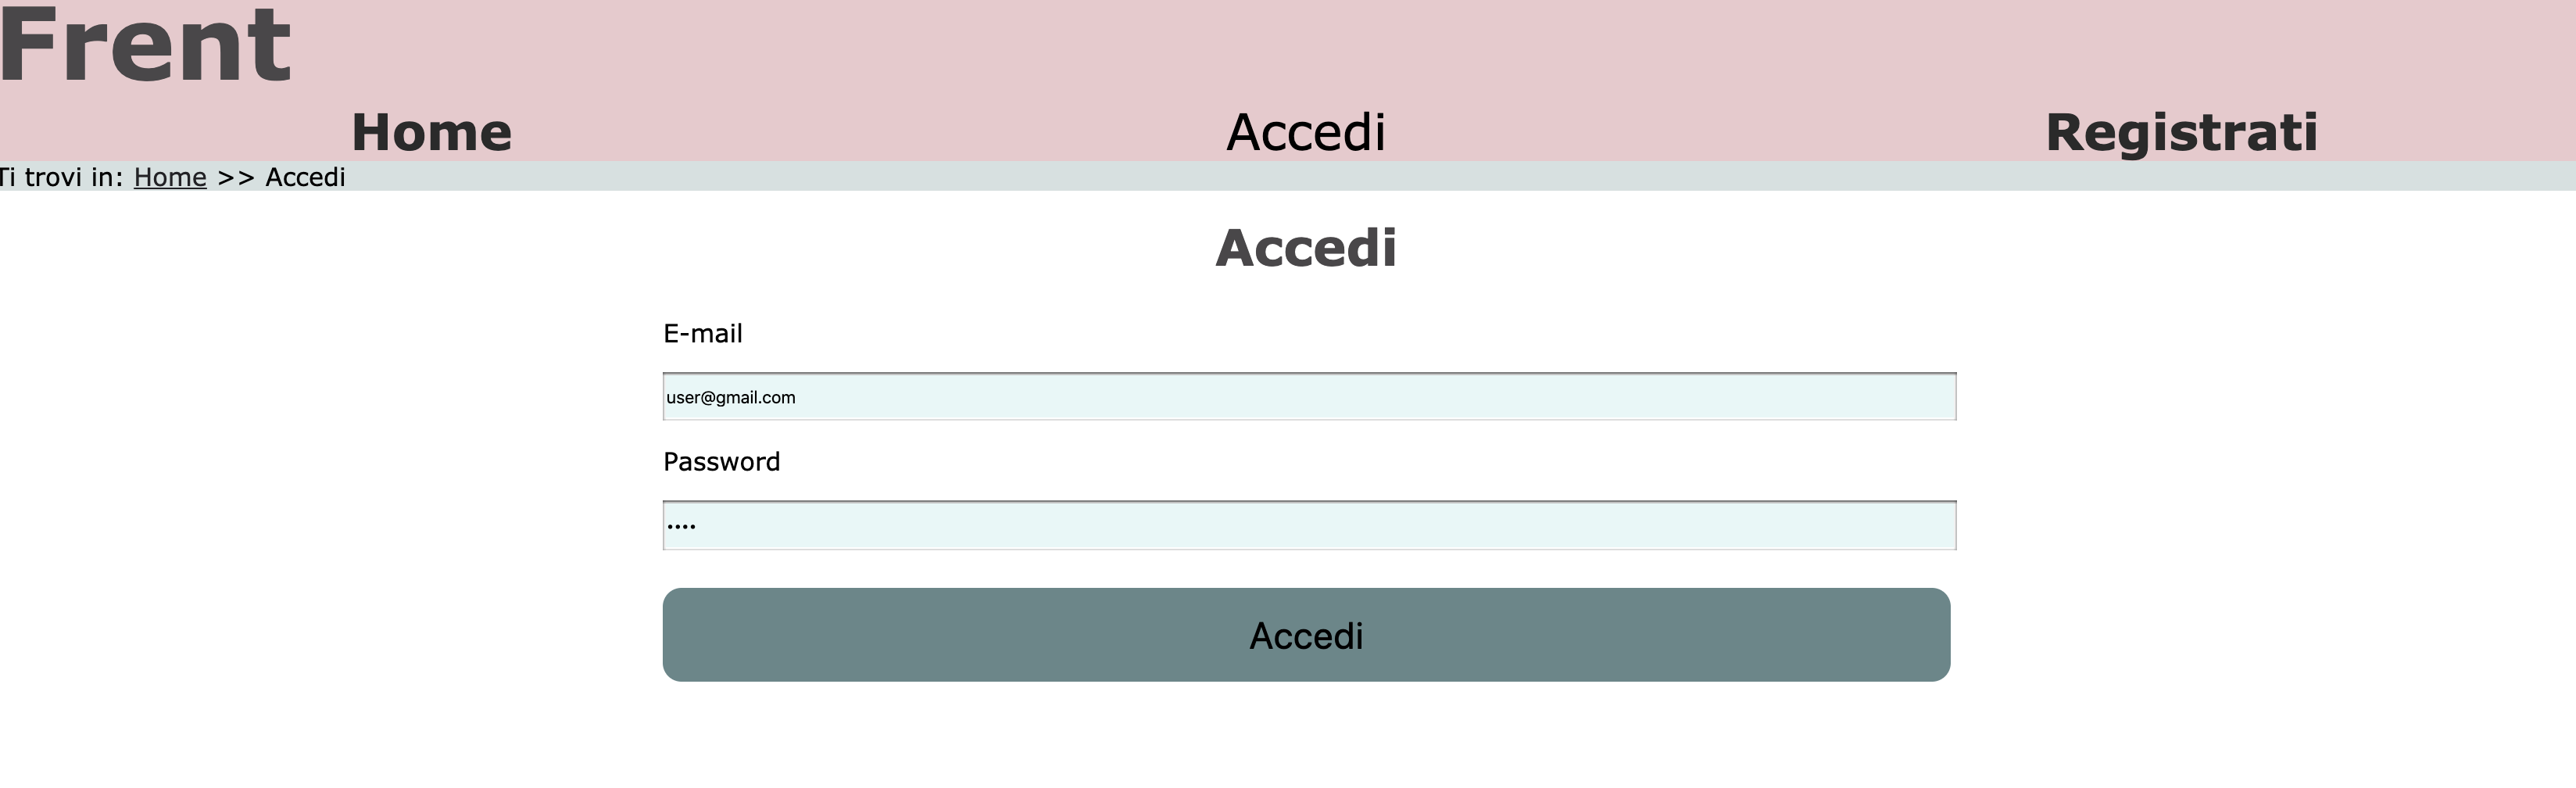
\includegraphics[scale=0.27]{immagini/Tritanopia.png}
        \caption{il sito visto da chi \`{e} affetto da tritanopia}
    \end{figure}

    \subsection{Inspect Code}
    \`{E} una funzionalit\`{a} di ispezione del codice sorgente offerta dall'IDE \textbf{PHPStorm}, che permette di elencare tutti gli errori di battitura e le eccezioni non gestite.

\end{document}
